% LaTeX report template 
%

% This is a comment: in LaTeX everything that in a line comes
% after a "%" symbol is treated as comment

\documentclass[11pt, a4paper]{article}
\usepackage{graphicx}
\usepackage{amsmath}
\usepackage{listings}


\title{\bold{\underline{\textit{\Large{Assignment 5: The Resistor Problem}}}}}

\author{ROHIT KUMAR [EE20B111]}

\date{March 11, 2021} 
\begin{document}	
		
\maketitle 
\section*{Abstract}
 The main goals of this assignment are :-
  \begin{itemize}
  \item
  	To show how currents depend on shape of resistor and the current's dependency on the shape of
the resistor and also which part of the resistor is likely to get hottest.
  \item
    To solve 2-D laplace equations using numerical approximation over a grid. how to vectorize in python code. To obtain the potential in the region by solving laplace's equation in 2-D and to plot graphs.
\end{itemize}  	
  
  \section{Introduction}
   We find the currents in the resistor after applying boundary conditions and analyse
the vector plot of current flow and conclude which part of resistor will
become hot. Resistors are used to reduce current flow, adjust signal levels, to divide voltages, bias active elements, and terminate transmission lines, among other uses.1In this assignment we intend to find the current density and potential gradient in a resistor.

	A  cylindrical wire is soldered to the middle of a copper plate and its voltage is held at 1 Volt.  One side of the plate is grounded, while the remaining are floating. The plate is 1 cm by 1 cm in size.\newline
We shall use these equations:\newline
The Continuity Equation:
\begin{equation}
    \nabla \cdot \vec{j} = - \frac{\partial\rho}{\partial t}
\end{equation}
Ohms Law:
\begin{equation}
    \vec{j} = \sigma\vec{E}
\end{equation}
The above equations along with the definition of potential as the negative gradient of Field give:
\begin{equation}
    \nabla^2 \phi =  \frac{1}{\rho}\frac{\partial\rho}{\partial t}
\end{equation}
For DC Currents, RHS of equation (3) is 0. Hence:
\begin{equation}
    \nabla^2 \phi =  0
\end{equation}
    
    
    \begin{itemize}
    \item
      Here we use a 2-D plate so the Numerical solutions in 2D can be easily
      transformed into a difference equation. The equation can be written
      out in
    \end{itemize}
    
    \begin{equation}
    \frac{\partial^{2} \phi}{\partial x^{2}}+ \frac{\partial^{2} \phi}{\partial y^{2}} = 0
     \end{equation}
    
    \begin{equation}
    \frac{\partial \phi}{\partial x}_{(x_i,y_j)} = \frac{\phi(x_{i+1/2},y_j) - \phi(x_{i-1/2},y_j)}{\Delta x}
     \end{equation}
    
    \begin{equation}
    \frac{\partial^{2} \phi}{\partial x^{2}}_{(x_i,y_j)} = \frac{\phi(x_{i+1},y_j) -2\phi(x_i,y_j)+ \phi(x_{i-1},y_j)}{(\Delta x)^{2}}
     \end{equation}
    
    \begin{itemize}
    \item
      Using above equations we get
    \end{itemize}
    
    \begin{equation}
            \phi_{i,j} = \frac{\phi_{i+1,j} + \phi_{i-1,j} + \phi_{i,j+1} + \phi_{i,j-1}}{4} 
    \end{equation}
    
    \begin{itemize}
    \item
     the solution at any point is a sum of values at neighbouring points.  The algorithm implemented makes use of the above equation to update $\phi$ over many iterations till it converges within an acceptable error.
  \end{itemize}

  \section{Defining Parameters and polential Array}
  

\begin{itemize}
\item
  Define the Parameters, The parameter values taken for my particular code were \(N_x = 25\) and \(N_y = 25\) and number of iterations : 1500
\item
  Allocate the potential array as \(\phi = 0\) .Note that the array
  should have \(N_y\) rows and \(N_x\) columns.
\item
  To find the indices which lie inside the circle of radius 0.35 using
  meshgrid() by equation :
\end{itemize}

\begin{equation}
X ^2 +Y ^2 \leq	 0.35^2
\end{equation}

\begin{itemize}
\item
  Then assign 1 V to those indices.

\end{itemize}

The python code snippet is as shown:
\begin{verbatim}
Nx = 25; 
Ny = 25; 
radius = 8;	
Niter = 1500;  

# Parameters given through command line
if(len(sys.argv) > 1 & len(sys.argv) < 4):
	Nx = int(sys.argv[1])
	Ny = int(sys.argv[2])
	Niter = int(sys.argv[3])
   
phi = zeros((Ny, Nx)) 
x = linspace(-0.5, 0.5, Nx) 
y = linspace(-0.5, 0.5, Ny)
n = array(range(Niter))
niter = arange(500, 1500, 0.1) 
X, Y = meshgrid(x, -y) 

# The coordinates can be found for points inside the given radius.
A = (X*X) + (Y*Y)
ii = where(A <= (0.35*0.35))

# Alloting the value of Phi as 1.0 at those coordinates.
phi[ii] = 1.0
figure(1)
semilogy(n,errors)
semilogy(n[::50], errors[::50], 'ro')
title("Error versus iteration")
xlabel(r'$Iteration\rightarrow$', size = 15)
ylabel(r'$Error\rightarrow$', size = 15)
grid(True)
       \end{verbatim}
       
The plot for the initial potential contour is as shown:
	     \begin{figure}[!tbh]
        \centering
        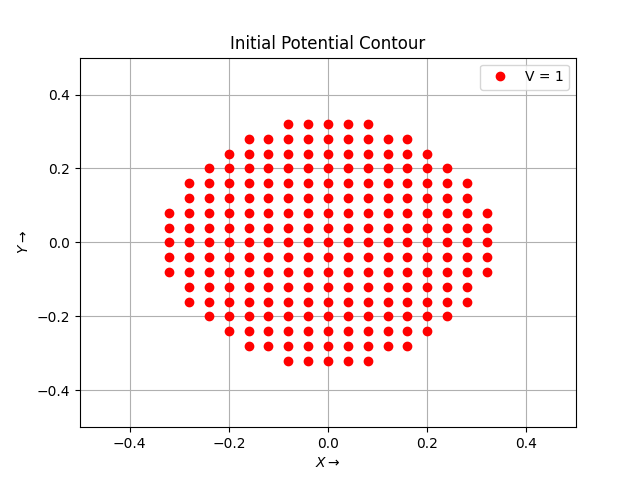
\includegraphics[scale=0.8]{Ass5_Figure_0.png}  
        \caption{Contour plot of initial potential}
   \end{figure}
 	\newpage
 \section{Performing the Iterations}
 \subsection{Updating Potential Array}

   \begin{itemize}
   
   \item
    Update the potential \(\phi\) according to Equation below using
     vectorized code
   \end{itemize}
   
   \begin{equation}
           \phi_{i,j} = \frac{\phi_{i+1,j} + \phi_{i-1,j} + \phi_{i,j+1} + \phi_{i,j-1}}{4} 
   \end{equation}
   
   \begin{itemize}
   \item
     To apply Boundary Conditions where there is no electrode, the gradient
     of \(\phi\) should be tangential. This is implemented by Equation
     given below , basically potential should not vary in the normal
     direction so we equate the last but row or column to outermost row or
     column correspondingly when applying boundary conditions for a side of
     plate,implemented using Vectorized code
   \end{itemize}
   
   \begin{equation}
    \frac{\partial \phi}{\partial n} = 0
   \end{equation}
 \subsection{Applying boundary conditions and Calculating error}
   
   The python code is as shown:-

   \begin{verbatim}
errors = empty((Niter, 1))
for k in range(Niter):
	oldphi = phi.copy()
	phi[1:-1, 1:-1] = 0.25*(phi[1:-1, 0:-2] + phi[1:-1, 2:] + phi[0:-2, 1:-1] + phi[2:, 1:-1])

# Applying the boundary conditions.
	phi[1:-1, 0] = phi[1:-1, 1]
	phi[1:-1, -1] = phi[1:-1, -2]
	phi[0, 1:-1] = phi[1, 1:-1]
	phi[ii] = 1.0
	errors[k] = (abs(phi - oldphi)).max()
    
         \end{verbatim}
 
 \section{The Error Estimations}  
 \begin{itemize}
 \item
 The error calculated can be analysed by plotting it against the iterations
 \item
 Using semilogy and loglog plots, For better visualisation consider only 50th point.
 \end{itemize}
\newpage 
 
The python code snippet for plotting the graphs are as shown:
 \begin{verbatim}
 
figure(1)
semilogy(n,errors)
semilogy(n[::50], errors[::50], 'ro')
title("Error versus iteration")
xlabel(r'$Iteration\rightarrow$', size = 15)
ylabel(r'$Error\rightarrow$', size = 15)
grid(True)

# Plotting of error vs iteration in loglog.
figure(2)
loglog(n,errors)
loglog(n[::50], errors[::50], 'ro')
title("Error versus iteration in a loglog plot")
xlabel(r'$Iteration\rightarrow$', size = 15)
ylabel(r'$Error\rightarrow$',size = 15)
grid(True)
\end{verbatim}       
\newpage
The respective error plots are as shown:

    
     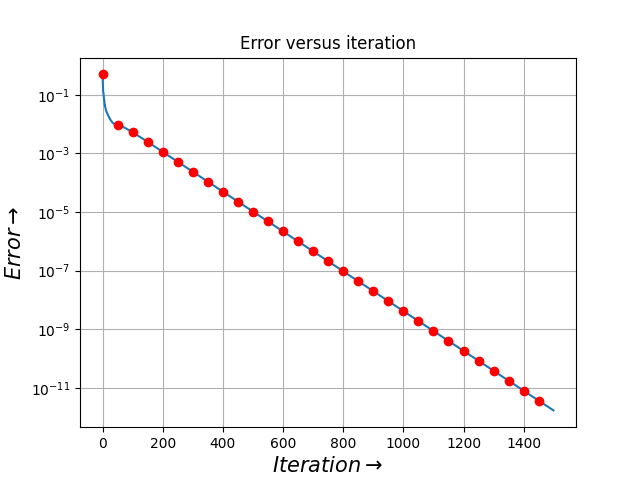
\includegraphics[scale=0.8]{Ass5_Figure_1.png} 
     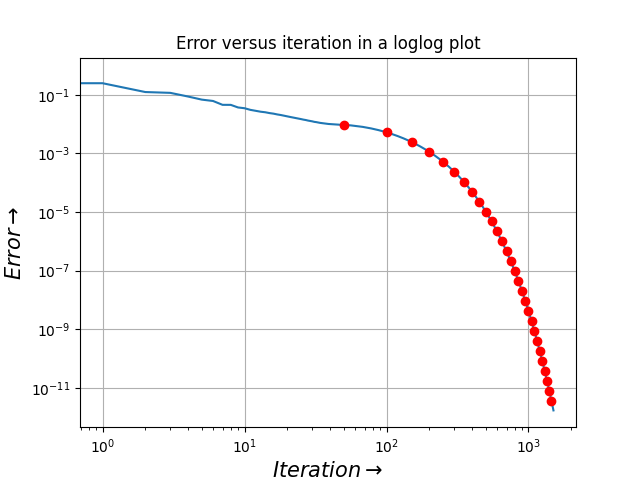
\includegraphics[scale=0.8]{Ass5_Figure_2.png}  



\subsection{Fitting the error}
We note that the error is decaying exponentially for higher iterations.I have plotted 2 fits. One considering all the iterations(fit1) and another without considering the first 500 iterations. There is very little difference between the two fits that too before 500 iterations. After 500th iteration there is no difference, Can be seen through comparing original and fit2.

The python code is as follows:-
\begin{verbatim}
def Fitting_Exp(x, A, B): # Defining the function Fitting_Exp(x, A, B)
    return A*np.exp(B*x) # Returning the value to A*np.exp(B*x) 
    
def Error_fitting(x, y): # Defining the function Error_Fitting(x, y) 
    logy = np.log(y)

    vector_x = np.zeros((len(x), 2))
    vector_x[:, 0] = x
    vector_x[:, 1] = 1
    B, logA = np.linalg.lstsq(vector_x, np.transpose(logy))[0]
    return (np.exp(logA), B)
    
c_approx_500 = lstsq(c_[ones(Niter - 500), array(range(500, Niter))], 
log(errors[500:]), rcond = None) 
A_500, B_500 = exp(c_approx_500[0][0]), c_approx_500[0][1]
print("The values of A and B for the iterations after 500 are: ", A_500, B_500)

c_approx = lstsq(c_[ones(Niter), array(range(Niter))], log(errors), rcond = None) 
A, B = exp(c_approx[0][0]), c_approx[0][1]
print("The values of A and B are: ", A, B)
    
fig3, ax1 = plt.subplots()
ax1.semilogy(range(Niter)[::50], errors[::50], label = 'original')
ax1.semilogy(range(Niter)[::50], Fitting_Exp(range(Niter)[::50], A, B), label = 'fit1')
ax1.semilogy(range(Niter)[::50], Fitting_Exp(range(Niter)[::50], A_500, B_500), label = 'fit2')
title("Best fit for error on semilog scale ")
xlabel(r'$Iteration\rightarrow$', size = 15)
ylabel(r'$Error\rightarrow$', size = 15)
grid(True)
legend()

fig4, ax2 = plt.subplots()
ax2.loglog(range(Niter)[::50], errors[::50], label = 'original')
ax2.loglog(range(Niter)[::50], Fitting_Exp(range(Niter)[::50], A, B), label = 'fit1')
ax2.loglog(range(Niter)[::50], Fitting_Exp(range(Niter)[::50], A_500, B_500), label = 'fit2')
title("Best fit for error on loglog scale ")
xlabel(r'$Iteration\rightarrow$', size = 15)
ylabel(r'$Error\rightarrow$', size = 15)
grid(True)
legend()


\end{verbatim} 


\begin{figure}[!tbh]
 \centering
 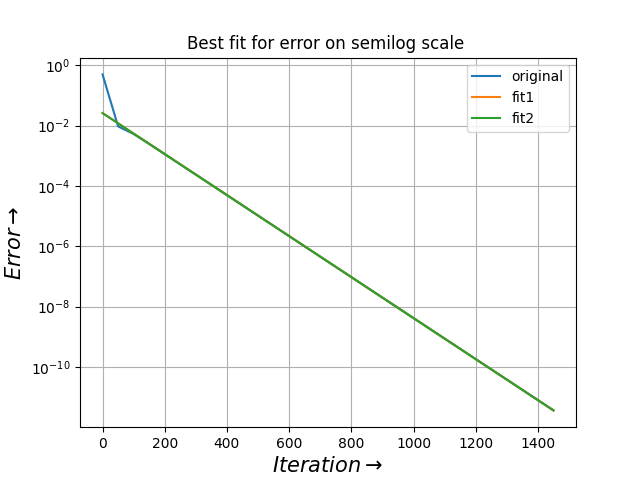
\includegraphics[scale=0.7]{Ass5_Figure_5.png}  
 \caption{Best fit of error}
\end{figure}

\begin{figure}[!tbh]
 \centering
 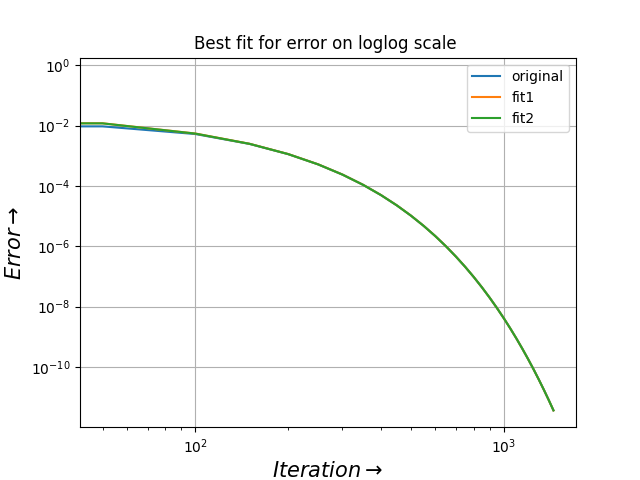
\includegraphics[scale=0.7]{Ass5_Figure_6.png}  
 \caption{best fit of error}
\end{figure}

\newpage
Upon execution of the code, we can get that 
\begin{itemize}
\item
$ A_{500} = 0.02604399$ and $B_{500} = -0.01564807 $ 

\item
$A = 0.02621557$ and $B = -0.01565526$

\end{itemize}


\section{Surface Plot of Potential}

We can analyse the potential variations by plotting it as a surface plot. The Python code is as follows:-
 \begin{verbatim}
fig1=figure(6)
ax = p3.Axes3D(fig1, auto_add_to_figure = False) 
fig1.add_axes(ax)
title("The 3-D surface plot of the potential")
xlabel(r'$X\rightarrow$')
ylabel(r'$Y\rightarrow$')
surf = ax.plot_surface(X, Y, phi, rstride = 1, cstride = 1, cmap = cm.jet)
fig1.colorbar(surf)
  \end{verbatim}
    

\newpage
The surface plot is as shown below:

\begin{figure}[tbh]
 \centering
 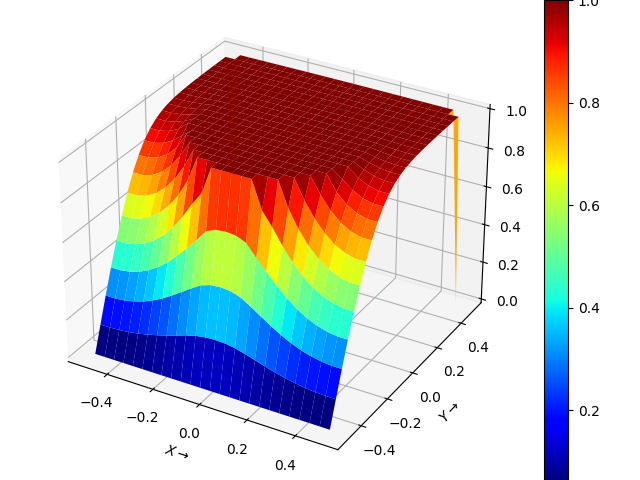
\includegraphics[scale=0.7]{Ass5_Figure_7.png}  
 \caption{3-D Surface potential plot of potential}
\end{figure}

\section{Contour Plot of the Potential}
We can analyse the potential variations by plotting it as a contour plot. The Python code is as follows:-
 \begin{verbatim}
 
figure(5)
contourf(X,Y,phi)
plot(ii[0]/Nx - 0.48, ii[1]/Ny - 0.48, 'ro', label = "V = 1")
title("Contour plot of potential")
xlabel(r'$X\rightarrow$')
ylabel(r'$Y\rightarrow$')
colorbar()
grid(True)
legend()
  \end{verbatim}

\begin{figure}[!tbh]
 \centering
 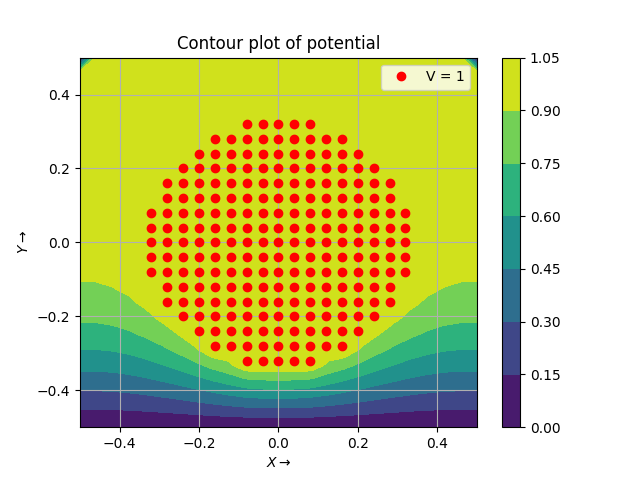
\includegraphics[scale=0.7]{Ass5_Figure_8.png}  
 \caption{Contour plot of potential}
\end{figure}
\newpage
\newpage

\section{Vector Plot of Currents}

\begin{itemize}
\item
  The currents in the system in Cartesian form can be expressed as :
\end{itemize}

\begin{equation}
    J_x = -\frac{\partial \phi}{\partial x} 
  \end{equation}

\begin{equation}
    J_y = -\frac{\partial \phi}{\partial y} 
  \end{equation}

\begin{itemize}
\item
  Numerically, this can be expressed as
\end{itemize}

\begin{equation}
        J_{x,ij} = \frac{1}{2}(\phi_{i,j-1} - \phi_{i,j+1}) 
    \end{equation}

\begin{equation}
        J_{y,ij} = \frac{1}{2}(\phi_{i-1,j} - \phi_{i+1,j}) 
    \end{equation}
  
The python code for calculating the the current densities and plotting is as follows:
   
  
\begin{verbatim}
Jx = zeros((Ny, Nx)) # Initialisation
Jy = zeros((Ny, Nx))
Jx[1:-1, 1:-1] = 0.5*(phi[1:-1, 0:-2] - phi[1:-1, 2:])
Jy[1:-1, 1:-1] = 0.5*(phi[2:, 1:-1] - phi[0:-2, 1:-1])
 
# plotting of the current vector plot along with the potential.
figure(7)
quiver(X, Y, Jx, Jy)
plot(ii[0]/Nx - 0.48, ii[1]/Ny - 0.48, 'ro')
title("Vector plot of the current flow")
xlabel(r'$X\rightarrow$')
ylabel(r'$Y\rightarrow$')
show()
  \end{verbatim}
The vector plot of the current flow along with the potential is as shown below:

  \begin{figure}[!tbh]
   \centering
   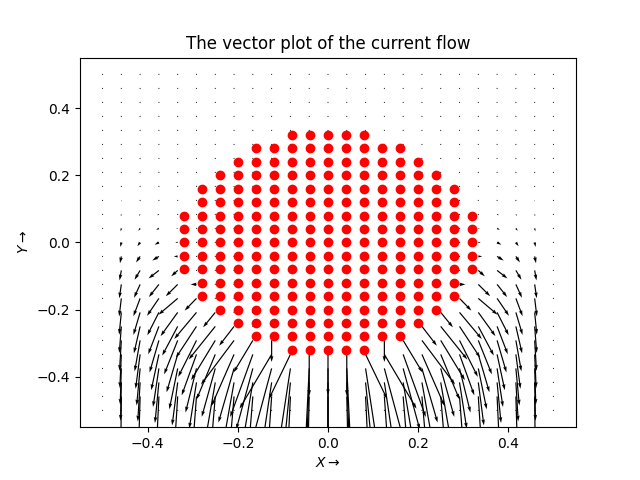
\includegraphics[scale=0.8]{Ass5_Figure_9.png}  
   \caption{Vector plot of current flow}
  \end{figure}
  

  \begin{itemize}
  \item
    So as we noted that the potential gradient was higher in down region
    of the plate, and we know that Electric field is the gradient of the
    potential as given below
  \end{itemize}
  
  \begin{equation}
  \vec{E} = -\nabla{\phi}
     \end{equation}
  
  \begin{itemize}
  \item
    So \(\vec{E}\) is larger where there is potential gradient is high and
    is inverted since it is negative of the gradient!, So it is higher in
    down region which is closer to bottom plate which is grounded
  \item
    And we know that
  \end{itemize}
  
  \begin{equation}
  \vec{J} = \sigma\vec{E}
     \end{equation}
  
  \begin{itemize}
  \item
    So \(\vec{J}\) is higher and perpendicular to equi-potential electrode
    region i.e "Red dotted region" so the current is larger in down part
    of the plate and perpendicular to the red dotted electrode region
    since \(I\) = \(\vec{J}.\vec{A}\)
  \item
   	we notice that hardly any current flows through  the  top  part  of  the  wire.   With  a  little  thought,  we  observe  that the lower surface being grounded, the easiest way for charge carriers to flow from the electrode would be directly through the lower half of the wire, thus avoiding a longer, more resistive path through the top half of the wire.
  \end{itemize}
  
    
  
    
      
  \section{Conclusion :}
  
  \begin{itemize}
  \item
  On analysing the quiver plot of the currents,  it was noticed that the current was mostly restricted to the bottom of the wire, and was perpendicular to the surface of the electrode and the conductor.
  \item
   The  currents  in  the  plate  are  normal  to  the  contour  lines.   In  addi-tion, most of the current flow is between the two electrodes with somefringing of the current near the edges
  \item
    Since there is almost no current in the upper region of plate, the
    bottom part of the plate gets hotter and temperature increases in down
    region of the plate.
  \item
    Very  little  current  flows  through  the  other  edges  of  the  plate.   This is primarily because most of the drop in the potential on the plate isb etween the central region and the top edge of the plate (as is clear from the surface plot).
  \item
    We observe that the best method to solve this is to
    increase \(N_x\) and \(N_y\) to very high values (100 or \(\geq\)
    100) and increase the number of iterations too, so that we get accurate
    answers i.e currents in the resistor.
  \item
  Using  a  finite  differentiation  approximation,  we  have  found  a  solution  toLaplace’s  equation  for  a  given  system.   The  error  is  seen  to  decay  at  ahighly gradual pace.  Thus the chosen method of solving Laplace’s equationis inefficient.
  \end{itemize}
  \end{document}